\chapter{Tensor Algebra}
\section{Introduction}\footnote{Notes taken from Introducing Einstein's relativity by Ray D'Inverno}
To work effectively in Newtonian theory, one reallyneeds the lenguage of vectors. This lenguage, first of all, is mire succint, since it  summarized a set of three equations in one. Moreoveer, the formalism of vectors helps to solver cartain problems more readly, adn, most important of all, the language reveals structure and thereby offers insight. In exactly the same way, in relativity theory, one needs the language of tensors. Again, the language helps to summarize sets of equations succintly and to solve problems more readly, and i reveals structure in the equaions. This part is devoted to learning the formalism of tensors shich is a pre-condition for the rest.

The approach we adopt is to concentrate on the technique of tensors without taking into account the deeper geometrical significance behind the theory. We shall be concerned more with whay you do with tensors rather than what tensors actually are. There are two distinct approaches to the teaching of tensors: the abstract or index-free (coordinate-free) approach and the conventional approach based on indices. There has been a move in recent years in some quarters to introduce tensors from the stars using the more mdodern abstract approach (although some have subsequantly changed their mind and reverted to the conventional approach). The main advantage of this approach is that it offers deeper geometrical insight. However, it has two disadvantages. First of all, it requieres much more of a mathematical background, which in turn takes time to develop. The other disadvantage is that, for all its elegance, when one wants to do real calculation with tensors, as one frequently needs to, then recourse has to be made to indices. We shall adopt the more conventional index approach, because ir will prove faster and more practical. However, we advise those who wish to take their study of the subject further to look at the index-free approach at the first oppoertunity.

\section{Manifolds and coordinates}

We shall start by working with tensors defined in $n$ dimensions since, and it is part of the power of the formalism, there is little extra effort involved. A tensor is an objet defined on a geometric entry called a (differential) \textbf{manifold}. We shall no define a manifold precisely because it would involve us too much of a digression. But, in simple terms, a manifold us simething which 'locally' looks like a bit of $n$-dimensional Euclidean space $\mathbb{R}^{n}$

We shall simply take an $n$-dimensional manifold $M$ to be a set of points such that each point posseses a set of $n$ \textbf{coordinates} $x^{1},x^{2},...,x^{n}$, where each coordinate ranges over a subset of the reals, which may, in particular, range from $-\infty$ to $+\infty$. To start off with, we can think of these coordinates as corresponding to distances or angles in Euclidean space. The reason why the cooridinates are written as superscrpts rather tan subscript will become clear later. Now the key thing about a manifold is that it may not be possible to cover the whole manifold by one \textbf{non-degenerate} cooridnate system, namely, one which ascribes a \textbf{unique} set of $n$ coorrdinate numbers to each point. Sometimes it is simply covenient to use coordinate numebrs to each point. Sometimes it is simply convenient to use coordinate systems with \textbf{degenerate} points. For example, plane polar coodinates $(R,\phi)$ in the plane have a degenneracy at the origin because $\phi$ is indeterminate there. However, here we could avoid the degeneracy at the origin by using Cartesian coordinates. But in other circumstances we have no choice in the matter. For example, it can be shown that there is no cooridate system shich covers the whole of a $2$.sphere $S^2$ without degeneracy. The smallest number is two. We therefore work with coordinate systems which cover only a portion of the manifold and which are called \textbf{cooridnate patches}. A set of cooridnate patches which covers the whole manifold is called an \textbf{atlas}. The theory of manifold tell us how to get from one coordinate patch to another by a coordinate transformation in the overlap region. The behaviour of geometric quantities under coodinate transformations lies at the heart of tensor calculus.

\section{Curves and surfaces}
We shall frequently define this curves and surfaces parametrically
\begin{equation}\label{5.1}
  x^{a} = x^{a}(u), \qquad a=1,...,n 
\end{equation}

\begin{equation}       \label{5.3}
  f(x^1,x^2,..., x^n)=0
\end{equation}
Points in an $m$-dimensional subsapce ($m<n$) must satisfy $n-m$ constraints
\begin{align}
\nonumber  f^1(x^1,...,x^n)=&0\\
\label{5.4}          &\vdots    \\
  \nonumber f^{n-m}(x^1,...,x^n)&=0
\end{align}

\section{Transformation of coordinates}
We need to find out how quantities behave when we go from one coordinate system to another one. We therefore consider the change of coordinates $x^{a}\to x'^{a}$ given by the $n$ equations
\begin{equation}\label{5.5}
  x'^{a}=f^{a}(x^1,...,x^n),\qquad a=1,...,n 
\end{equation}
we can write (\ref{5.5}) more succintly as $x'^{a}=f^{a}(x)$ , or more simply
\begin{equation}        \label{5.6}
  \boxed{x'^{a}=x^{a}(x)}
\end{equation}
We next contemplate differentiating (\ref{5.6}) with respect to each coordinates $x^b$
\begin{equation*}
  \left[\pdv{x'^{a}}{x^b}\right] 
\end{equation*}
the determinant $J'$ of this matrix is called the \textbf{Jacobian} of the transformation 
\begin{equation}                   \label{5.8}
  J'=\left|\pdv{x'^{a}}{x^b}\right|
\end{equation}
Assume that thus is non-zero. Then we can solve (\ref{5.6}) for the old coordinates $x^{a}$ and obtain the \textbf{inverse} transformation
\begin{align*}
  x^{a}&=x^{a}(x)\\
  J&=\left|\pdv{x^{a}}{x'^b}\right| \qquad (\mbox{Jacobian of the inverse transformation})\\
  J&=\frac{1}{J'}
\end{align*}
In 3 dimensions, the equation of a surface is given by $z=f(x,y)$, then its total differential is defined to be
\begin{equation*}
  \dd z =\pdv{f}{x}\dd x + \pdv{f}{y}\dd y
\end{equation*}
Then, in an analogus manner, starting from (\ref{5.6}) we define the total differential 
\begin{equation*}
  \dd x'^{a}=\pdv{x'^{a}}{x^1}\dd x^1+\cdots +\pdv{x'^{a}}{x^n}\dd x^n
\end{equation*}
\begin{equation}                                   \label{5.10}
  \dd x'^{a} =\sum_{b=1}^n\pdv{x'^{a}}{x^b}\dd x^b 
\end{equation}
introducing the \textbf{Einstein summation convention}
\begin{equation}                   \label{5.11}
  \boxed{\dd x'^{a}=\pdv{x'^{a}}{x^b}}
\end{equation}
It defines the Kronecker delta as
\begin{equation}
  \delta_b^{a}=\left\{ \begin{array}{lc}
    1 ,& a=b\\
  0 ,& a\neq b\end{array}\right.
\end{equation}
It therefore follow directly from the definition of partial differentiaton that
\begin{equation}                                \label{5.13}
  \pdv{x'^{a}}{x'^b}=\pdv{x^{a}}{x^b}=\delta_b^{a}
\end{equation}

\section{Contravariant tensors}\label{sec:5.5}
We shall start with a prototype and then give general definition.

Consider two neighboring points in the manifold $P$ and $Q$ with coordinates $x^{a}$ and $x^{a}+\dd x^{a}$  respectively. The two points define an \textbf{infinitesimal displacement} or \textbf{infinitesimal vector} $\overrightarrow{PQ}$. The components of this vector in the $x^{a}$-coordinate system are $\dd x^{a}$. The components in another coordinate system, say the $x'^{a}$-coordinate system, are $\dd x'^{a}$ which are conected to $\dd x^{a}$ by (\ref{5.11})
\begin{equation}\label{4.14}
  \dd x'^{a}=\pdv{x'^{a}}{x^b}\dd x^b
\end{equation}
The transformation matrix appearing in this equation is to be regarded as being evaluated at the point $P$, i.e, strictly speaking we should write 
\begin{equation}\label{5.15}
  \dd x'^{a}=\left[\pdv{x'^{a}}{x^b}\right]_P\dd x^b 
\end{equation}
A \textbf{contravariant vector} or \textbf{contravariant tensor of rank (order) 1} is a set of quantities, written $X^{a}$ in the $x^{a}$-coordinates system, associated with a point $P$, which trasform under a change of coordinates according to
\begin{equation}\label{5.16}
  \boxed{X'^{a}=\pdv{x'^{a}}{x^b}X^b }
\end{equation}
where the transform matrix is evaluated at $P$. The infinitesimal vector $\dd x^{a}$ is a special case of (\ref{5.16}) where the components $X^{a}$ are infinitesimal. 

A \textbf{contravariant tensor of rank 2} es a set of $n^2$ quantities associated with a point $P$, denoted by $X^{ab}$ in the $x^{a}$-coordinate system, which transform according to 
\begin{equation}\label{5.17}
  X'^{ab}=\pdv{x'^{a}}{x^c}\pdv{x'^b}{x^d}X^{cd }
\end{equation}
An important case is a tensor of zero rank, called a \textbf{scalar} or \textbf{scalar invariant} $\phi$, which transform according to 
\begin{equation}\label{5.18}
  \boxed{\phi' =\phi}
\end{equation}
at $P$.

\section{Covariant and mixed tensors}
Let
\begin{equation}\label{5.19}
  \phi=\phi(x^{a})
\end{equation}
be a real-valued function on the manifold (at every point $P$ in the manifold, $\phi(P)$ produces a real number). Also assume that $\phi$ is continuous and differentiable.

Remembering from (\ref{5.9}), $x^{a}$ can be thought of as a function of $x'^b$, (\ref{5.19}) can be written equivalently as $$\phi=\phi(x^{a}(x'))$$ Remembering Differentiating this with respect to $x'^b$, we obtain 
\begin{equation*}
  \pdv{\phi}{x'^b}=\pdv{\phi}{x^{a}}\pdv{x^{a}}{x'^b }
\end{equation*}
Then changing the order of the terms, the dummy index, and the free index (from $b$ to $a$) gives
\begin{equation}\label{5.20}
  \pdv{\phi}{x'^{a}}=\pdv{x^b}{x'^{a}}\pdv{\phi}{x^b }
\end{equation}
This is the prototype equation we are looking for. Notice that it involves the inverse transformation matrix $\pdv*{x^b}{x'^{a}}$. Thus, a \textbf{convariant vector} or \textbf{covariant tensor of rank (order) 1} is a set of quantities, which transform according to 
\begin{equation}\label{5.21}
  \boxed{X'_a=\pdv{x^b}{x'^{a}}X_b}
\end{equation}
Again, the transform matrix occuring is assumed to be evaluated at $P$.

Similary, we define a covariant tensor of rank 2 by the transform law
\begin{equation}\label{5.22}
  X'_{ab} = \pdv{x^c}{x'^a}\pdv{x^d}{x'^b}X_{cd}
\end{equation}
and so on for higher-rank tensors.

Note the convention that contravariant tensors have raised indices whereas covariant tensors have lowed indices. The way to remember this is the \textbf{co} goes \textbf{below}. The fact that the differentials $\dd x^{a}$ transform as a contravariant vector explains the convention that the coordinate  themeselves are written as $x^{a}$ rather than $x_a$, although note that it is only the differentials and not the coordinates which have tensorial character. 

We can go on on to define \textbf{mixed} tensors in the obvious way. For example, a mixed tensor of rank 3- one contravariant rank and two covariant rank- satisfies
\begin{equation}\label{5.23}
  X'^{a}_{bc}=\pdv{x'^{a}}{x^d}\pdv{x^{e}}{x'^{b}}\pdv{x^f}{x'^{c}}X^{d}_{ef}
\end{equation}
If  a mixed tensor has contravariant rank $p$ and covariant rank $1$, then it is said to have \textbf{type} or \textbf{valence} $(p,q)$. 

Suppose we find in one coordinate system that two tensors, $X_{ab}$ and $Y_{ab}$ say, are equal 
\begin{equation}\label{5.24}
  X_{ab}=Y_{ab}
\end{equation}
Les us multiply both sides by the matrices $\pdv*{x^{a}}{x'^c}$ and $\pdv*{x^b}{x'^c}$ and take the implies summations to get
\begin{equation*}
  \pdv{x^{a}}{x'^c}\pdv{x^b}{x'^d}X_{ab}=\pdv{x^{a}}{x'^c}\pdv{x^b}{x'^d}Y_{ab}
\end{equation*}
Since $X_{ab}$ and $Y_{ab}$ are both covariant tensors of rank 2 it follows that $X'_{ab}=Y'_{ab}$. In other words, (\ref{5.24}) holds in \textbf{any} other coordinate system. In short, a tensor equations whics holds in one coordinate system necessarily holds in \textbf{all} coordinate systems. Thus, although we introduce coordinate systems for convenience un tackling particular problems, if we work with tensorial equations then they hold in all coordinate systems. Put another way, tensorial equations are coordinate-independet. This is something that the index-free or coordinate-free approach makes clear from the outset.

\section{Tensor Fields}\label{sec:5.7}
In a vector analysis, a fixed is a vector associated with a point, whereas a vector \textbf{field} defined over a region is an association of a vector to every point in that region. In exactly the same way, a tensor is a set of quantities defined at one point in the manifold. A \textbf{tensor field} defined over some region of the manifold is an assocaition of a tensor of the same valence to every point of the region, i.e: $$P\to T_{b...}^{a...}(P)$$ where $T_{b...}^{a...}(P)$ is the value of the tensor at $P$. The tensor fields is called continous or differentiable if its components in all cordinate systems are continuous  or differentiable functions of the cooridinates. The tensor field is called smooth if its components are differentiable to all orders, which is denoted mathematically by saying that all the components are $C^\infty$. Thus, for example, a contravariant vector fields defined over a region is a set of $n$ \textbf{functions} defined over that region, and the vector field is \textbf{smooth} if the functions are all $C^\infty$. The transformation law for contravariant vector field then becomes
\begin{equation}\label{5.25}
  X'^{a}(x')=\left[\pdv{x'^{a}}{x^b}\right]_PX^b(x)
\end{equation}
at each point $P$ in the region, since the old components $X^{a}$ are functions of the old $x^{a}$-coordinates and the new components $X'^{a}$ are funxtions of the new $x'^{a}$-coordinates.

As in the case of vectors and vector fields in vector analysis, the distinction between a tensor and a tensor field is not always made completely clear. We shall for the most part be dealing with tensor field from now on, but to confo, whith general usage we shall often refer to tensor fields simply as tensors. We will again shorten the transformation law such as (\ref{5.25}) to the form (\ref{5.21}) with everything else being implied. If we wish to emphasize that a tensor is a field. we shall write it in functional form, namely, as $T_{b...}^{a...}(x)$.

\section{Elementary Operations with Tensors}\label{sec:5.8}
Tensor calculus is concernerd with \textbf{tensorial operations}, that is, operations on tensors which result in quantities which are still tensors. A simple way of establishing whether or not a quatity is a tensor is to see how it transform under a coordinate transformation. For example, we can deduce directly from the transformation law that two tensors of the same type can be added together to give a tensor of the same type, e.g.
\begin{equation}\label{5.26}
  \tensor{X}{^{a}_{bc}} = \tensor{Y}{^{a}_{bc}} + \tensor{Z}{^{a}_{bc}}
\end{equation}
The same holds true for subtraction and scalar multiplication.

A covariant tensor of rank $2$ is said to be \textbf{symmetric} if $X_{ab}=X_{ba}$, in which case it has only $\frac{1}{2}n(n+1)$ independent components (check this by establishing how many independent components there are of a symmetric matrix of order $n$). Symmetry is a tensorial property. A similar definition holds for a contravariant tensor $X^{ab}$. The tensor $X_{ab}$ is said to be \textbf{ant-symmetric} or \textbf{skew symmetric} if $X_{ab}=-X_{ba}$, which has only $\frac{1}{2}n(n-1)$ independent components; this is again a tensorial property. A notation frequantly used to denote the symmetric part of a tensor is
\begin{equation}\label{5.27}\marginnote{Symmetric part of a tensor}
  X_{(ab)}=\frac{1}{2}(X_{ab}+X_{ba})
\end{equation}
and the anti-symmetric part is
\begin{equation}\label{5.28}\marginnote{Anti-symmetric part of a tensor}
  X_{[ab]}=\frac{1}{2}(X_{ab}-X_{ba})
\end{equation}
In general, 
\begin{equation}
  X_{(a_1a_2\cdots a_r)}=\frac{1}{r!}\quad\mbox{(sum over all permutations of the indices $a_1$ to $a_r$)}
\end{equation}
and
\begin{equation}
  X_{[a_1a_2\cdots a_r]}=\frac{1}{r!}\quad\mbox{alternating sum over all permutations of the indices $a_1$ to $a_r$}
\end{equation}
For example, we shall ned to make use of the result
\begin{equation}\label{5.29}
  X_{[abc]}=\frac{1}{6}(X_{abc}-X_{axb}+X_{cab}-X_{cba}+X_{bca}-X_{bac})
\end{equation}
(A way to remember the above expression is to note that the positive terms are obtained by cycling the indices to the right and the corresponding negative terms by flipping the last two indices.) A \textbf{totally symmetric tensor} os defined to be one equal to its symetric part, and a \textbf{totally anti-symmetric tensor} is one equal to its anti-symmetric part.

We can multiply two tensors of type $(p_1,q_1)$ and $(p_2,q_2)$ together and obtain a tensor of type $(p_1+p_2, q_1+q_2)$, e.g.
\begin{equation}\label{5.30}
  \tensor{X}{^{a}_{bcd}}=\tensor{Y}{^{a}_b}\tensor{Z}{_{cd}}
\end{equation}
In particular, a tensor of type $(p,q)$ when multiplied by a scalar field $\psi$ is again a tensor of type $(p,q)$. Given a tensor of mixed type $(p,q)$, we can form a tensor of type $(p-1,q-1)$ by the procces of \textbf{contraction}, which simply involves setting a raised and lowering index equal. For example,
\begin{equation*}
  \tensor{X}{^{a}_{bcs}}\xrightarrow{\mbox{contraction on $a$ and $b$}}\tensor{X}{^{a}_{acd}}=Y_{cd}
\end{equation*}

\section{Index-free Interpetration of Contrvariant Vector Fields}\label{sec5.9}
As we pointed out in \ref{sec:5.5}, we must distinguish between the actual geometric object otself and its components on a particular coordinate system. The important point about tensors is that we want to make statements shich are independent of any particular coordinate system being used. This si abundatly clear in the idnex-free approach to tensors. We shall get a feel for this approach in this section by sonsidering the special case of a contravariant vector field, althought similar idnex-free interpretations can be given for any tensor field. The key idea is to interpret the vector field as an \textbf{operator} which maps real-valued functions into real-valued functions. Thus, if $X$ represents a contravariant vector field, then $X$ operates on any real-valued function $f$ to produce another function $g$, i.e. $Xf=g$. We shall show how actually to compute $Xf$ by introducing a coordinate system. However, as we shall see, we could equally well introduce any other coordinate system, and the computation would lead to the same result.

In the $x^{a}$--coordinate system, we introduce the notation $$\partial_a\equiv\frac{\partial}{\partial x^{a}}$$ and the $X$ is defined as the operator
\begin{equation}\label{5.32}
  \boxed{X=X^{a}\partial _a}
\end{equation}
\begin{equation}\label{5.33}
  Xf=(X^{a}\partial_a)f=X^{a}(\partial _a f)
\end{equation}
for any real-valued function $f$. Let us compute $X$ in some other $x'^{a}$-coordinate system. We need to use the result (\ref{5.13}) expressed in the following form: we may take $x^{a}$ to be a function of $x'^b$ by (\ref{5.9}) and $x'^b$ to be a function of $x^c$ by (\ref{5.6}), and so, using the function of a function rule, we find
\begin{equation}\label{5.34}
  \delta^{a}_b=\pdv{x^{a}}{x^b}=\frac{\partial}{\partial x^b}x^{a}(x'^c(x^d))=\pdv{x^{a}}{x'^c}\pdv{x'^c}{x^b}
\end{equation}
Then, using the tranformation law (\ref{5.16}) and (\ref{5.20}) together with the above trick, we get
\begin{align*}
  X'^{a}\partial '_a&=X'^{a}\frac{\partial}{\partial x'^{a}}\\
                    &=\pdv{x'^{a}}{x^b}X^b\pdv{x^c}{x'^{a}}\frac{\partial}{\partial  x^c}\\
                    &=\pdv{x^c}{x'^{a}}\pdv{x'^{a}}{x^b}X^b\frac{\partial}{\partial x^c}\\
                    &=\delta^{a}_bX^b\frac{\partial}{\partial x^c}\\
                    &=X^b\frac{\partial}{\partial x^b}\\
                    &=X^{a}\frac{\partial}{\partial x^{a}}\\
                    &=X^{a}\partial_a
\end{align*}
Thus the result of operating on $f$ by $X$ will be the same \textbf{irrespective} of the coodinate system employed in (\ref{5.32}).

In any coordinate system, we may think of the quantities $[\partial/\partial x_a]_P$ as forming a basis for all the vectors at $P$, since any vector at $P$ i, by (\ref{5.32}), given by $$X_P=[X^{a}]_P\left[\frac{\partial}{\partial x^{a}}\right]_P$$ that is, a linear combination of the $[\partial/\partial x^{a}]_P$. the vector space of all the contravariant vectors at $P$ is known as the \textbf{tangent space} of $P$ and is written $T_P(M)$. (Fig. \ref{fig:5.6}). In general, the tangent space at any point in a manifold is different from the underlying manifold. For this reason, we need to be careful in repesenting a finite contravariant vector by an arrow in our figures since, strictly speaking, the arrow lies in the tangent space not the manifold. Two exceptions to this are Euclidean space and Minkowski space-time, where the tangent space at each point coincides with the manifold.
\begin{figure}[h!]
	\begin{center}
		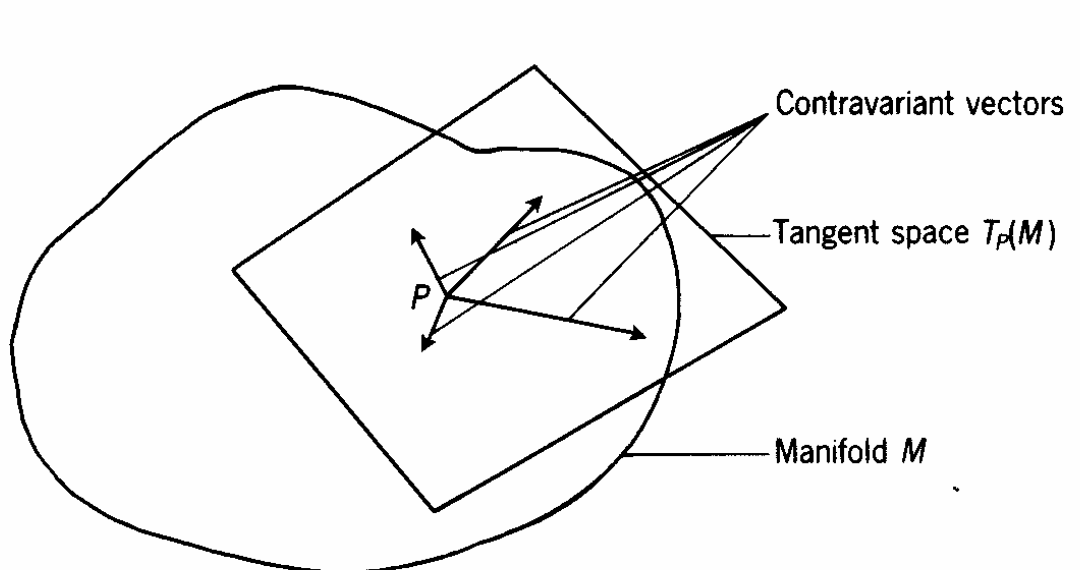
\includegraphics[scale=0.4]{fig/fig:5-6.png}
    \caption{The tangent space at $P$.}
    \label{fig:5.6}
	\end{center}	
\end{figure}

Given two vector fields $X$ and $Y$ we can define a new vector field called the \textbf{commutator} or \textbf{Lie bracker} of $X$ and $Y$ by
\begin{equation}\label{5.35}\marginnote{Lie bracket}
  \boxed{[X,Y]=XY-YX}
\end{equation}
Letting $[X,Y]=Z$ and operating with it on some arbitrary dunction $f$
\begin{align*}
  Zf&=[X,Y]f\\
    &=(XY-YX)f\\
    &=X(Yf)-Y(Xf)\\
    &=X(Y^{a}\partial_af)-Y(X^{a}\partial_af)\\
    &=X^b\partial_b(Y^{a}\partial_af)-Y^b\partial_b(X^{a}\partial_af)\\
    &=(X^b\partial_bY^{a}-Y^b\partial_bX^{a})\partial_af-X^{a}Y^b(\partial_b\partial_af-\partial_a\partial_bf)
\end{align*}
The least term vanishes since we assume commutativity of second mixed partial derivatives, i.e. $$\partial_a\partial_b=\frac{\partial^2}{\partial x^{a}\partial x^b}=\frac{\partial^2}{\partial x^b\partial x^{a}}=\partial_b\partial_a$$ Since $f$ is arbitrary, we obtain the result
\begin{equation}\label{5.36}
  [X,Y]^{a}=Z^{a}Z^b\partial_bY^{a}-Y^b\partial_bX^{a}
\end{equation}
from which it crealy follows  that the commutator of two vector fields is itself a vector field. It also follows. directly from de definition (\ref{5.35}), that
\begin{equation}\label{5.37}
  [X,X]\equiv 0
\end{equation}
\begin{equation}\label{5.38}
  [X,Y]\equiv [Y,X]
\end{equation}
\begin{equation}\label{5.39}
  [X,[Y,Z]] + [Z,[X,Y]] + [Y,[Z,X]]\equiv 0
\end{equation}
(\ref{5.38}) shows that the Lie bracker is ant-commutative. The result (\ref{5.39}) is known as \textbf{Jacobi's identity}. Notice it states that the ledt-hand side is not just equal to zero but is \textbf{identically} zero. What does it mean? The equation $x^2-4=0$ is only satisfied by particular values of $x$, namely, $+2$ and $-2$. The identity $x^2-x^2\equiv 0$ is satisfied for all vallues of $x$. But, you may argue, the $x^2$ terms cancel out, and this is precisely the point. An expression is identically zero if, when all the terms are written out fully, they all cancel in pairs.








